\subsubsection{Presentation Layer}
Tầng presentation có mục đính chính là biểu diễn những giao diện mà chúng tôi
muốn thiết kế, nó sẽ bao gồm những hàm là những tính năng chính của trang đó.

\begin{figure}[H]
    \centering
    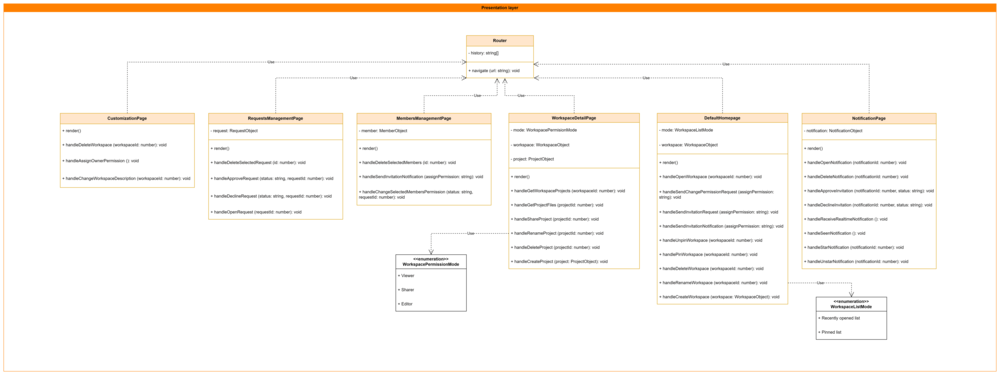
\includegraphics[ width = \linewidth]{Content/Phân tích và thiết kế hệ thống/documents/Sơ đồ lớp/images/Presentation layer/presentationLayer.png}
    \vspace{0.5cm}
    \caption{Presentation Layer}
    \label{fig:Presentation layer}
\end{figure}

\begin{figure}[H]
    \centering
    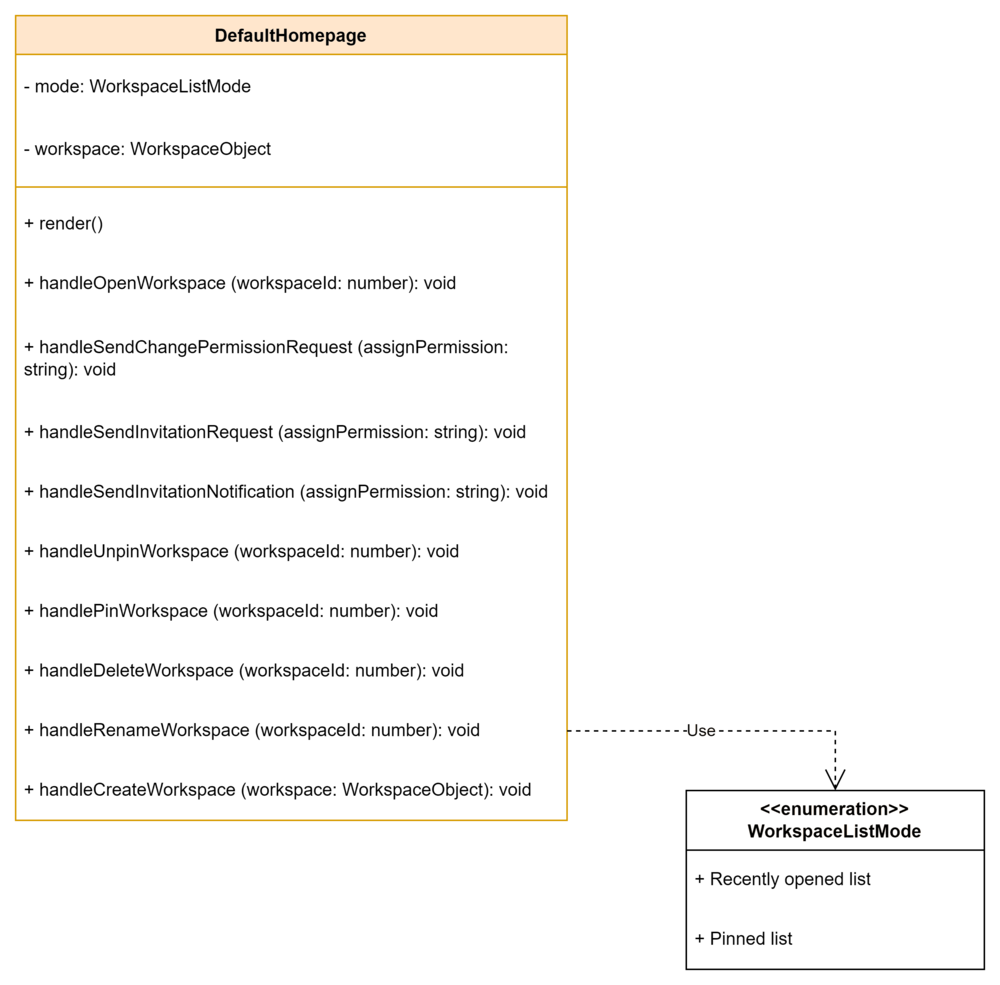
\includegraphics[ width = \linewidth]{Content/Phân tích và thiết kế hệ thống/documents/Sơ đồ lớp/images/Presentation layer/defaultWorkspacePage.png}
    \vspace{0.5cm}
    \caption{Default homepage trong Presentation layer}
    \label{fig:Default homepage trong Presentation layer}
\end{figure}

\begin{figure}[H]
    \centering
    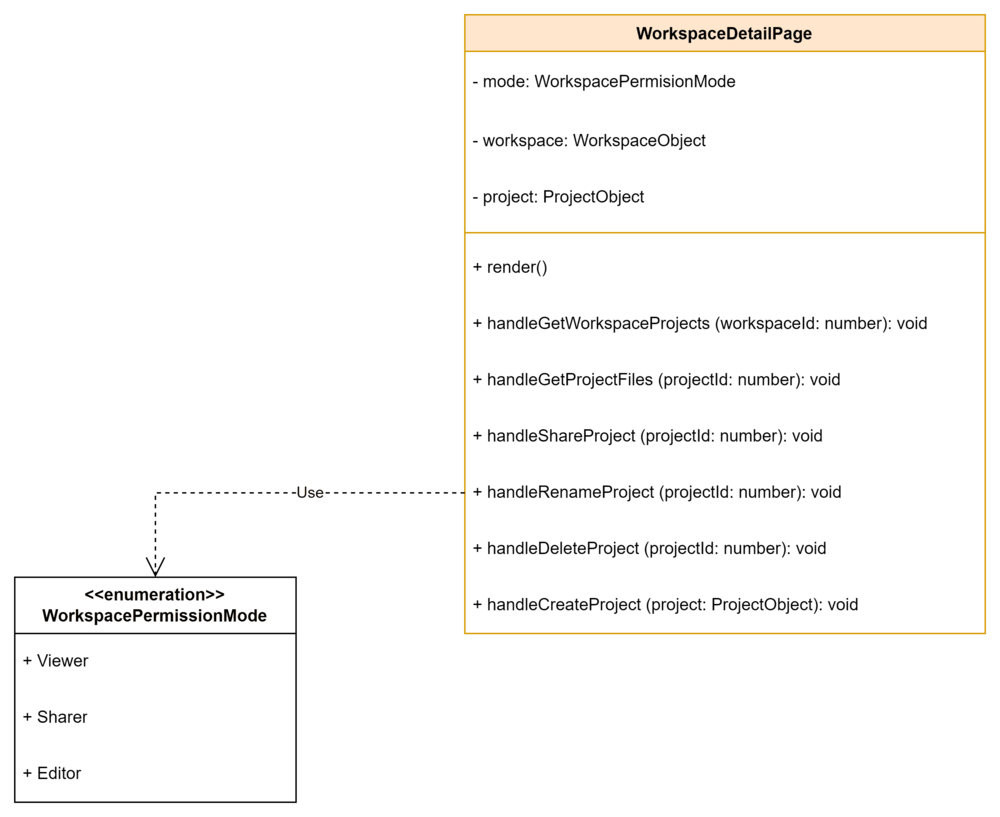
\includegraphics[ width = \linewidth]{Content/Phân tích và thiết kế hệ thống/documents/Sơ đồ lớp/images/Presentation layer/workspaceDetailPage.png}
    \vspace{0.5cm}
    \caption{Workspace detail page trong Presentation layer}
    \label{fig:Workspace detail page trong Presentation layer}
\end{figure}

\begin{figure}[H]
    \centering
    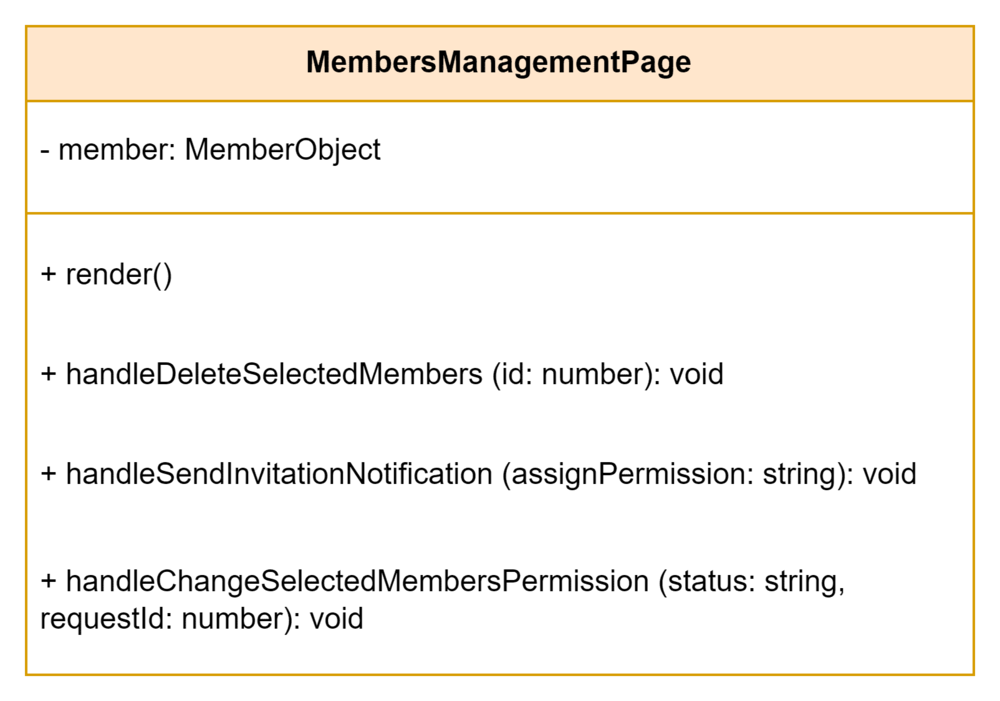
\includegraphics[ width = \linewidth]{Content/Phân tích và thiết kế hệ thống/documents/Sơ đồ lớp/images/Presentation layer/membersManagementPage.png}
    \vspace{0.5cm}
    \caption{Member management page trong Presentation layer}
    \label{fig:Member management page trong Presentation layer}
\end{figure}

\begin{figure}[H]
    \centering
    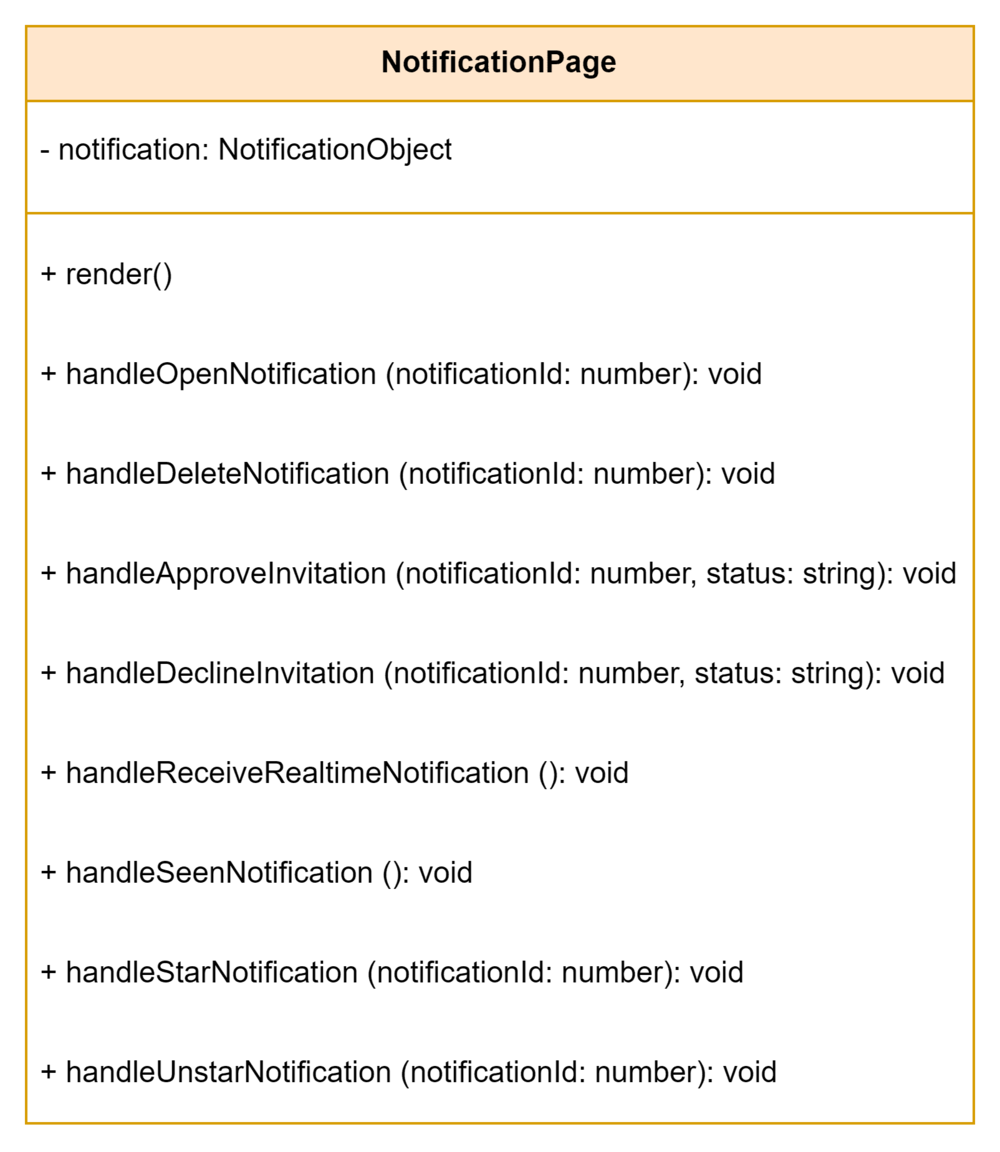
\includegraphics[ width = \linewidth]{Content/Phân tích và thiết kế hệ thống/documents/Sơ đồ lớp/images/Presentation layer/notificationPage.png}
    \vspace{0.5cm}
    \caption{Notification page trong Presentation layer}
    \label{fig:Notification page trong Presentation layer}
\end{figure}

\begin{figure}[H]
    \centering
    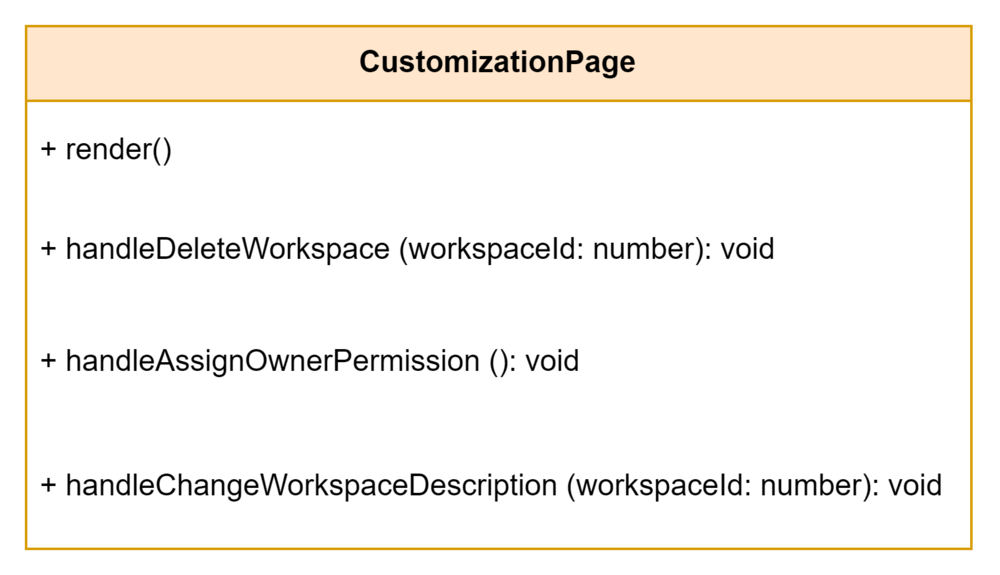
\includegraphics[ width = \linewidth]{Content/Phân tích và thiết kế hệ thống/documents/Sơ đồ lớp/images/Presentation layer/customizationPage.png}
    \vspace{0.5cm}
    \caption{Customization page trong Presentation layer}
    \label{fig:Customization page trong Presentation layer}
\end{figure}

\begin{figure}[H]
    \centering
    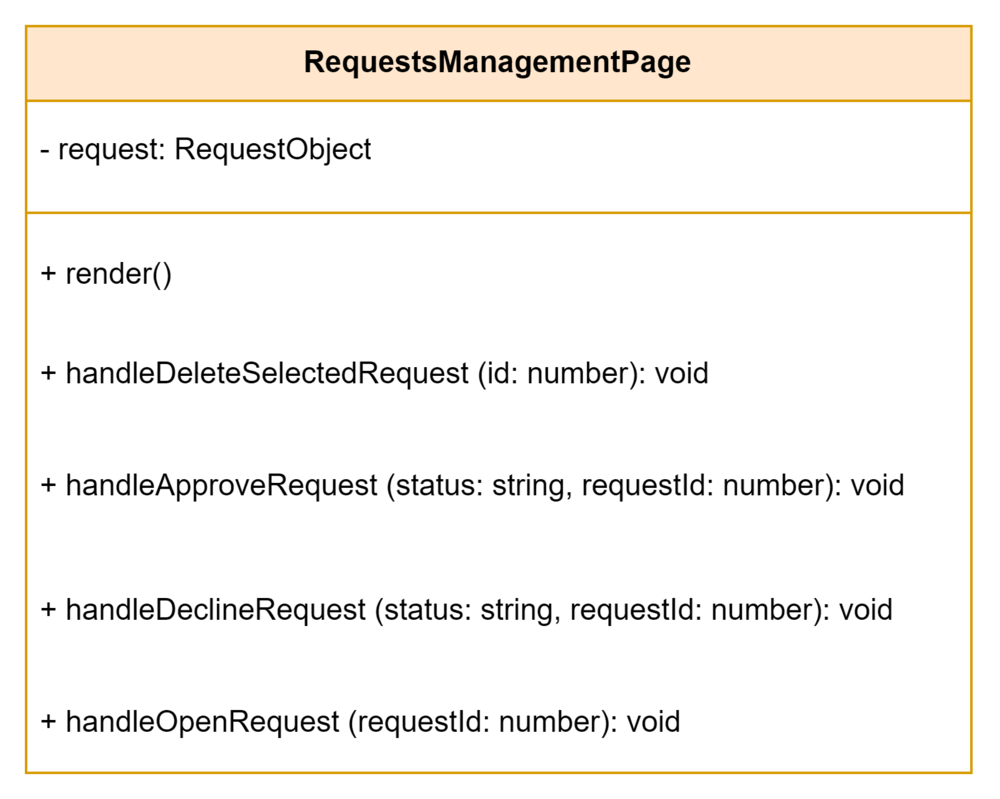
\includegraphics[ width = \linewidth]{Content/Phân tích và thiết kế hệ thống/documents/Sơ đồ lớp/images/Presentation layer/requestManagementPage.png}
    \vspace{0.5cm}
    \caption{Request management page trong Presentation layer}
    \label{fig:Request management page trong Presentation layer}
\end{figure}